\documentclass[varwidth]{standalone}
\usepackage{tikz}

\begin{document}

    \begin{figure}[h!]
        \centering
        
        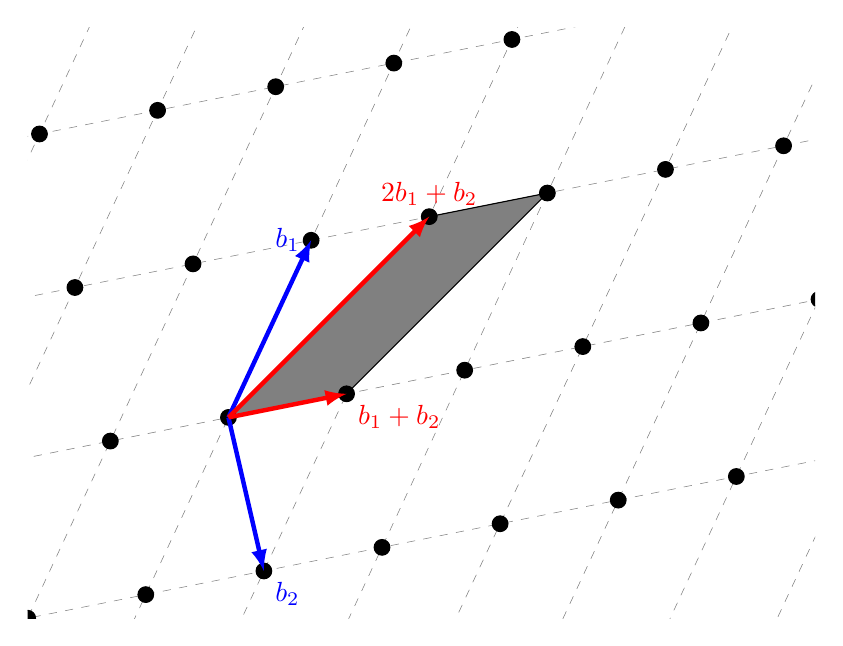
\begin{tikzpicture}[>=latex]
        
            \begin{scope}
                % Clips the global figure
                \clip (0, 0) rectangle (10cm, 7.5cm);

                % Performs the transformation on the global figure,
                % including rotation and translation
                \pgftransformcm{1}{0.2}{0.7}{1.5}{\pgfpoint{0cm}{0cm}}

                 % Draws a dashed helper grid in the new coordinates
                \draw[style=help lines,dashed] (-14,-14) grid[step=1.5cm] (14,14);

                % Draws the shaded region between the shortest vectors and bases used
                \filldraw[fill=gray, draw=black] (1.5,1.5) --  (3,3) -- (4.5,3) -- (3,1.5) -- cycle;

                % For each point in the x-axis of coordinates
                \foreach \x in {-7,-6,...,7} {
                
                    % For each point in the y-axis of coordinates
                    \foreach \y in {-7,-6,...,7} {
                    
                        % Draws a node on the grid at the (x,y) points
                        \node[draw,circle,inner sep=2pt,fill] at (1.5*\x,1.5*\y) {};
                    
                    }
                
                }

                % Draws the vector for the bases choices
                \draw[ultra thick,blue,->] (1.5,1.5) -- (1.5,3) node [left] {$b_1$}; 
                \draw[ultra thick,blue,->] (1.5,1.5) -- (3,0) node [below right] {$b_2$};
                \draw[ultra thick,red,->] (1.5,1.5) -- (3,3) node [above] {$2b_1+b_2$}; 
                \draw[ultra thick,red,->] (1.5,1.5) -- (3,1.5) node [below right] {$b_1+b_2$}; 
                
            \end{scope}
            
        \end{tikzpicture}
    
    \end{figure}

\end{document}